\newpage

\section{Dataset}

The dataset used for this project was a competition dataset from Hugging Face, held in 2023 \cite{huggingface_competitions_aiornot}.
The dataset consists of 62,060 images, and is 2.37GB in size, being pre-split into training and tesing sets, as summarised in \cref{tab:dataset_summary,tab:class_counts}, where it can be seen that the testing set has the class labels withheld due to the competition setting, restricting this analysis to the 18,618 training images, which we can sub-divide and validate with known labels.
\begin{table*}[h]
    \centering
    \begin{minipage}{0.48\textwidth}
        \centering
        \begin{tabular}{ll}
            \toprule
            \textbf{Feature} & \textbf{Description} \\
            \midrule
            \code{id}     & Index filename \code{34.jpg} \\
            \code{image}  & The Image (512x512) \\
            \code{label}  & Binary class label \\
            \bottomrule
        \end{tabular}
        \caption{Dataset features and their descriptions.}
        \label{tab:dataset_summary}
    \end{minipage}\hfill
    \begin{minipage}{0.48\textwidth}
        \centering
        \begin{tabular}{lcc}
            \toprule
            \begin{tabular}[c]{@{}l@{}}\textbf{Class} \\ \textbf{Label}\end{tabular} & 
            \begin{tabular}[c]{@{}c@{}}\textbf{Train} \\ \textbf{Count}\end{tabular} & 
            \begin{tabular}[c]{@{}c@{}}\textbf{Test} \\ \textbf{Count}\end{tabular} \\
            \midrule
            AI (1)      & 10,330 $(55.5\%)$ & NA \\
            Not AI (0)  & 8,288 $(45.5\%)$ & NA \\
            \bottomrule
            \textbf{Total}       & 18,618 & 43,442 \\
        \end{tabular}
        \caption{Counts of each class label in the training and testing sets}
        \label{tab:class_counts}
    \end{minipage}
\end{table*}

\Cref{code:data_wrangling} shows the code used to load the dataset, and split it into training, validation, and test sets. It can be seen that the splitting method for the data was to 
- holdout 500 images for final testing (only 500 was chosen due to a bandwidth issue on the AWS endpoint, further elaborated on in \Cref{sec:model_deployment}),
- split the remaining training data into three sets, the small train, train and test set, being 10\%, 70\%, and 20\% of the remaining data respectively.
- to ensure class balance between these sets, random oversampling was employed. This was because \cref{tab:class_counts} shows that if a model were to guess AI all the time, it could get an accuracy of 55.5\%

\Cref{code:data_wrangling}, in the appendix shows the code used to load the dataset from HuggingFace. It can then be seen that the splitting sceme described above is done using hugging faces \code{train_test_split} method. The HuggingFace dataset object is converted to numpy arrays. Then \code{Imblearn}'s \code{RandomUnderSampler} is used to ensure class balance, as to not bias the majority class.



This data was converted to npz files, due to their efficient storage and loading capabilities. After conversion, the data was uploaded to an S3 bucket for easy access during model training and evaluation. Uploading to S3 buckets was critical, as it meant that there was no longer a reliance on the RAM allocation of the sagemaker notebook environment - it could be loaded in from the S3 bucket in batches, which has the benefit of being a more scalable solution.

\begin{figure}[h]
    \centering
    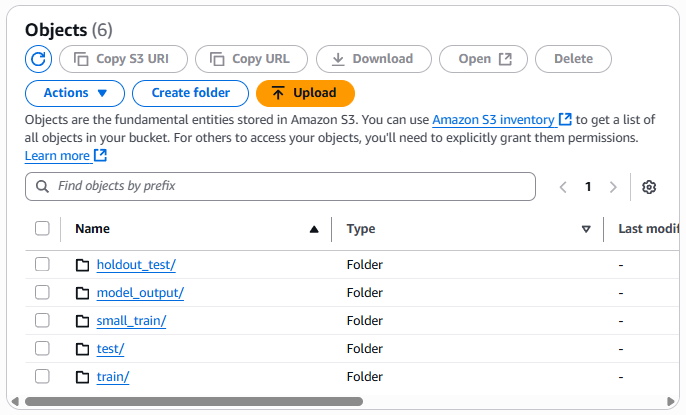
\includegraphics[width=200px]{figures/s3_bucket_screenshot.png} % Image filename
    \centering
    \caption{Screenshot of S3 Bucket in AWS Console} % Caption
    \label{fig:s3_bucket} % Label
\end{figure}


